\documentclass[conference]{IEEEtran}
\IEEEoverridecommandlockouts
\usepackage{cite}
\usepackage{amsmath,amssymb,amsfonts}
\usepackage{algorithm}
\usepackage{algpseudocode}
\usepackage{graphicx}
\usepackage{textcomp}
\usepackage{xcolor}
\usepackage{booktabs}
\usepackage{tikz}
\usetikzlibrary{arrows.meta,positioning,fit,backgrounds}
\usepackage{hyperref}
\usepackage{url}

\def\BibTeX{{\rm B\kern-.05em{\sc i\kern-.025em b}\kern-.08em
    T\kern-.1667em\lower.7ex\hbox{E}\kern-.125emX}}

\begin{document}

\title{OpsPilot+: Implementing and Evaluating Three Named-but-Unbuilt\\
Research Directions for Multi-Agent Legacy Toolchain Modernization}

\author{
\IEEEauthorblockN{Sumit V Togarshi}
\IEEEauthorblockA{Dept. of Comp. Sci. \& Eng.\\
HKBK Institute of Technology\\
Bengaluru, India\\
1hk23cs163@hkbk.edu.in}
\and
\IEEEauthorblockN{Suprith S Naik}
\IEEEauthorblockA{Dept. of Comp. Sci. \& Eng.\\
HKBK Institute of Technology\\
Bengaluru, India\\
1hk23cs166@hkbk.edu.in}
\and
\IEEEauthorblockN{Sunil I M}
\IEEEauthorblockA{Dept. of Comp. Sci. \& Eng.\\
HKBK Institute of Technology\\
Bengaluru, India\\
1hk23cs164@hkbk.edu.in}
\linebreakand
\IEEEauthorblockN{Saksham Arya}
\IEEEauthorblockA{Dept. of Comp. Sci. \& Eng.\\
HKBK Institute of Technology\\
Bengaluru, India\\
1hk23cs134@hkbk.edu.in}
\and
\IEEEauthorblockN{Prof. Tahir Naquash}
\IEEEauthorblockA{Dept. of Comp. Sci. \& Eng.\\
HKBK Institute of Technology\\
Bengaluru, India\\
tahir.cs@hkbk.edu.in}
}

\maketitle

\begin{abstract}
A companion survey examined multi-agent orchestration for legacy toolchain
modernization and proposed OpsPilot, a four-phase conceptual reference
architecture, while explicitly noting that OpsPilot itself was not
implemented or empirically evaluated. That survey also named three specific
capabilities as open, unbuilt gaps in the surveyed literature: guardrail
thresholds that adapt from human-override history rather than staying fixed
(``guardrail stagnation,'' identified as the AI-guardrails framework's own
stated primary limitation), a self-refine iteration budget that adapts
per-module rather than using one fixed value for an entire migration run, and
persistent, repository-scale project memory with propagation-aware
re-verification. This paper reports an actual implementation. We build
OpsPilot as runnable, tested Python code with a deterministic four-phase
pipeline, then implement three additive extensions closing the three named
gaps: SentinelPolicy, a Thompson-sampling contextual bandit that learns
per-risk-category guardrail thresholds without ever touching a non-learned
hard-constraint layer; RefineRL, a predictor-plus-online-adjuster that sets
and revises a per-module self-refine iteration budget; and RepoMind, a
persistent dependency graph and semantic memory store with a change-propagation
agent that schedules targeted re-verification. All three are evaluated with
reproducible, code-driven experiments on synthetic benchmarks calibrated to
the companion survey's own reported figures. SentinelPolicy reduces
wasted-escalation rate by 95.3\% relative to a static threshold while
preserving a 100\% hard-constraint catch rate. RefineRL lands near, but not
strictly above, the cost/convergence-rate frontier traced by fixed iteration
budgets on the same benchmark -- a result we report honestly rather than
reframe. RepoMind achieves 100\% recall of truly-impacted downstream modules
while reducing re-verification scope by 67\% relative to re-verifying an
entire repository. We report these results with the same evidentiary
discipline as the source survey: every figure here comes from code that
actually ran, distinguished throughout from the directions we deliberately
did not implement and why.
\end{abstract}

\begin{IEEEkeywords}
Multi-Agent Systems, Large Language Models, Legacy Code Modernization,
Contextual Bandits, Adaptive Guardrails, Iteration Budget Allocation,
Repository-Scale Memory, Change Propagation, Software Engineering
\end{IEEEkeywords}

\section{Introduction}

Multi-agent orchestration for legacy toolchain modernization has, per a
recent structured survey of 30 primary sources across IEEE Xplore, the ACM
Digital Library, and arXiv, matured into a coherent methodology with named
components: an Analysis/Discovery agent, an Orchestrator, a Coder/Verifier
self-refine loop, and a Governance layer \cite{survey}. That survey
synthesized these components into OpsPilot, a four-phase conceptual reference
architecture, while being explicit that OpsPilot itself ``has not been
implemented or empirically evaluated'' and that its contribution was ``a
shared vocabulary for future empirical work, not independent evidence of
feasibility'' \cite{survey}.

This paper is that future empirical work. We implement OpsPilot as an
actual, tested, runnable system, and then extend it with three research
directions the survey names explicitly as unsolved rather than directions we
independently identified:

\begin{itemize}
\item \textbf{Guardrail stagnation.} The survey's own comparative table lists
``overly strict rules cause guardrail stagnation'' as the stated primary
limitation of the AI-guardrails framework it surveys \cite{survey}, and its
future-work section proposes ``adaptive, sensitivity-based guardrail
thresholds \ldots via policy-gradient methods'' without anyone having built
one.
\item \textbf{Fixed self-refine iteration budgets.} Section VI of the survey
reports that convergence ``typically converges within 3--5 iterations for
well-structured COBOL modules but may need up to 12 for modules with embedded
SQL or CICS handlers, motivating an adaptive rather than fixed iteration
budget $B$'' \cite{survey} -- again, named directly, never built, in any
surveyed system.
\item \textbf{Repository-scale project memory.} Section V-A of the survey
admits its own Orchestrator's shared project-memory store is ``a target
design goal \ldots rather than a proven one,'' and Section VII flags
``global refactoring, where one module's change must propagate consistently
across hundreds of dependents'' as technically unsolved due to context-window
constraints \cite{survey}.
\end{itemize}

We call the resulting system OpsPilot+. Section \ref{sec:base} describes the
base four-phase implementation. Section \ref{sec:extensions} describes the
three extensions -- SentinelPolicy, RefineRL, and RepoMind -- and,
consistent with the source survey's own transparency about what a related
gap-analysis process surfaced but this project chose not to pursue, explains
which of ten candidate research directions we implemented and which we
deliberately excluded, and why. Section \ref{sec:methodology} describes our
evaluation methodology. Section \ref{sec:results} reports results, including
one that is a genuine trade-off rather than a clean win, reported as such.
Section \ref{sec:threats} discusses threats to validity. Section
\ref{sec:future} outlines future work, and Section \ref{sec:conclusion}
concludes.

\textbf{Contributions.} (1) A working, tested, four-phase implementation of
the OpsPilot reference architecture, previously conceptual only. (2)
SentinelPolicy, RefineRL, and RepoMind: three additive extensions, each
targeting a gap the source survey names explicitly, each implemented as real
code with unit tests and wired into the live pipeline behind feature flags.
(3) Reproducible, code-driven evaluation of all three against principled
baselines, including an explicit accounting of where results are clean wins
and where they are genuine, unresolved trade-offs. (4) A documented account
of research directions considered and deliberately not implemented, and why
-- including one (adaptive agent-topology selection) that we found to
directly conflict with a design constraint of the base architecture itself.

\section{Background}

We do not re-survey the literature the companion paper already covers in
depth \cite{survey}; we summarize only what this paper builds on directly.
Conversable agents and conversation programming, as formalized in AutoGen
\cite{autogen}, let LLM instances exchange structured turns under a
controlling Orchestrator rather than free-form dialogue. The self-refine
cycle -- a Coder proposes, a Verifier critiques, the Coder revises -- descends
from Self-Refine \cite{selfrefine} and Reflexion's episodic-memory extension
\cite{reflexion} of the ReAct reasoning-acting loop \cite{react}, and is the
mechanism every surveyed migration pipeline uses for iterative code
correction, always under one fixed iteration budget. AI guardrails, per
Mishra's framing \cite{guardrails}, are structured technical, ethical, and
regulatory controls that bound agent behavior; the surveyed implementations
of this idea are uniformly deterministic and non-learning.

Two general-purpose techniques underpin our extensions without themselves
being migration-specific contributions. Upper-Confidence-Bound and
Thompson-sampling algorithms address the explore/exploit trade-off in
multi-armed bandit problems \cite{ucb, thompson1933, thompsontutorial};
LinUCB extends this to contexts with side information via ridge-regression
reward estimation per arm \cite{linucb}. We use these as the learning
mechanism inside SentinelPolicy, applying them to a problem -- guardrail
threshold calibration for code-migration governance -- that, to our
knowledge, is not addressed in the bandit literature or the migration
literature it currently sits adjacent to.

\section{Base System: OpsPilot Implemented}
\label{sec:base}

The base implementation follows the four phases and four non-negotiable
design constraints specified by the source survey's reference architecture
\cite{survey}: (1) legacy source is never sent to an LLM for structural
parsing -- deterministic Python parsers extract JSON-Schema-validated
summaries first; (2) no flat multi-agent group chat -- a deterministic Python
control plane sequences phases explicitly; (3) the self-refine inner loop is
strictly two agents (Coder, Verifier) under a hard iteration budget; (4)
safety and governance checks are hardcoded, deterministic Python functions
registered as a message interceptor, never an LLM asked to judge its own
safety.

Phase 1 (Discovery) uses deterministic parsers for COBOL and PL/SQL source,
producing a schema-validated analysis summary and a per-module dependency
graph via NetworkX. Phase 2 (Orchestration) is a single-shot call to an
Analysis Agent that proposes a Java object-oriented design roadmap from the
Phase 1 summary. Phase 3 (Execution) runs a bounded Coder/Verifier self-refine
loop implementing Eq.~1 of the source survey, terminating on convergence or
budget exhaustion. Phase 4 (Governance) registers a deterministic guardrail
interceptor at position zero on the Verifier agent, checking every proposed
change against a fixed denylist (destructive DDL, command injection,
credential leakage, unauthorized process control) before any execution
side-effect occurs. Because this environment has no LLM API credentials, the
implementation includes an offline, deterministic stand-in for the underlying
agent-conversation library that reproduces its message-passing interface, so
the full pipeline runs end-to-end and is unit-testable without network
access; every extension in Section \ref{sec:extensions} is designed to
function identically whether the underlying Coder/Verifier calls a real LLM
or this deterministic stand-in, since none of the three touch code
generation itself.

\section{OpsPilot+ Extensions}
\label{sec:extensions}

\subsection{Scope: what we built, and what we deliberately did not}
\label{sec:scope}

Ten candidate research directions were considered for this project, four
sketched at gap-analysis depth and three specified to full research-proposal
depth. We implemented the three fully-specified directions --
SentinelPolicy, RefineRL, and RepoMind -- and deliberately excluded four
others. We report this decision explicitly, in the same spirit as the source
survey's own transparency about its screening process, rather than silently
narrowing scope.

One exclusion is architectural, not a matter of priority: an
adaptive-topology-selection direction, in which a meta-orchestrator would
learn to choose among two-agent, sequential, nested, and group-chat
topologies per subtask, directly contradicts Constraint 2 of the base
architecture (no flat group chat, a single deterministic control plane by
design). Implementing it inside this codebase would mean arguing against the
base architecture's own stated design commitment within the same repository
that enforces it; it belongs in a different reference architecture, not
bolted on quietly. A second candidate, a risk-calibrated guardrail-threshold
idea sketched independently, turned out on inspection to describe the same
mechanism as SentinelPolicy at lower specification depth; we implemented the
fully-specified version once rather than building the same bandit-over-thresholds
system twice under two names, and treat one of its distinguishing details --
asymmetric updates that auto-tighten freely but require human sign-off to
loosen -- as a documented future extension (Section \ref{sec:future}) rather
than part of the present system. The remaining two exclusions, adaptive
human-review-checkpoint placement and reinforcement-learning-based model-tier
routing across agent roles, were both judged legitimate and were cut for
scope: three ideas implemented rigorously, with real bugs found and fixed
and honestly reported evaluation, was judged a better outcome than five
implemented shallowly.

\subsection{SentinelPolicy: Adaptive Guardrail Thresholds}
\label{sec:sentinel}

\subsubsection{Design}
SentinelPolicy adds a second governance layer alongside -- never inside --
the existing deterministic denylist. The denylist (hard constraints: schema
DDL, credential access, process/command execution) remains untouched,
non-learned Python pattern matching, exactly as in the base system; every
SentinelPolicy decision checks it first and short-circuits before any
learned component is consulted. Alongside it, SentinelPolicy scores generated
code against seven graduated soft-risk categories that were never part of
the hard denylist -- financial-precision (floating-point used for monetary
fields instead of fixed-precision arithmetic), null-safety, resource
management, exception handling, deprecated-API usage, magic numbers in
business logic, and unbounded loops -- via regex-density heuristics, weighted
by a module's declared risk class (financial, utility, or standard).

For each (risk category, module risk class) pair, a discrete ladder of
threshold candidates is learned via Beta--Bernoulli Thompson sampling
\cite{thompson1933, thompsontutorial}, one of the two bandit formulations the
underlying idea specification names as acceptable (the other, LinUCB
\cite{linucb}, is also implemented and available as a pluggable alternative,
but a shared-context regression is a worse fit here than a small set of
near-stationary per-group bandits: each group's reward distribution is
governed by a roughly fixed human-override tendency for that category, not a
continuously-varying function of the score itself, which favors classical
multi-armed bandit convergence over cross-context generalization). Given a
risk score $s$ and Thompson-sampled threshold $t$ for a category's group:

\begin{equation}
\text{decision} =
\begin{cases}
\text{APPROVE} & s < t - m \\
\text{REJECT} & s > t + m \\
\text{ESCALATE} & \text{otherwise}
\end{cases}
\end{equation}

\noindent where $m$ is a fixed escalation margin. Every human disposition
(simulated, for evaluation purposes; see Section \ref{sec:methodology}) on
an ESCALATE or REJECT decision updates that category's Beta posterior:
success (reward 1) if the human's disposition agreed with the policy's
implicit call, failure (reward 0) otherwise. Critically, this reward is
recorded \emph{per category}, not aggregated across all categories flagged
in a single module -- an early implementation bug, discovered during
development and documented in Section \ref{sec:threats}, aggregated a
module's seven category dispositions into one AND'd boolean before
recording, which let one unrelated flagged category poison the learning
signal for six well-calibrated ones.

\subsection{RefineRL: Predictive Iteration-Budget Allocation}
\label{sec:refinerl}

\subsubsection{Design}
RefineRL wraps budget logic around the existing Coder/Verifier loop without
altering the loop's mechanics. A Pre-Refinement Predictor -- a
gradient-boosted regressor, with a closed-form ridge-regression fallback when
scikit-learn is unavailable -- maps Discovery-time features (embedded-SQL
flag, CICS-handler flag, a call-graph-density cyclomatic-complexity proxy,
dependency count) to a starting iteration budget, trained on logged
(features, actual-iterations) pairs from prior runs. A Trajectory Monitor
then tracks the Verifier-reported failure count $\delta_t$ after each
iteration and classifies it as improving, converged, or plateaued:

\begin{equation}
\text{plateau at } t \iff \delta_{t-w} \le \delta_t \;\wedge\; \delta_{t-w} \neq 0
\end{equation}

\noindent over a window $w$ -- deliberately a strict ``no net progress at
all'' criterion rather than a small-relative-improvement threshold, because a
softer criterion is unreliable against integer-valued, slowly-decaying
failure counts, as detailed in Section \ref{sec:threats}. A Dynamic Budget
Adjuster then acts on this signal: convergence ends the loop; a detected
plateau triggers early human-in-the-loop escalation regardless of remaining
budget, rather than grinding to the original limit; a trajectory still
genuinely improving when the budget is nearly exhausted is granted a bounded
extension rather than cut off; and a trajectory converging unusually fast has
its remaining budget shortened. This last mechanism required a
reliability guard: relative-improvement spikes caused by ordinary integer
rounding of small counts (a drop from 3 to 1 is a ``67\% improvement'' but is
rounding noise, not evidence of unusually fast convergence) are excluded by
requiring the pre-drop count to exceed a minimum threshold before the
adjuster will shorten the budget on that signal.

\subsection{RepoMind: Persistent Memory and Change Propagation}
\label{sec:repomind}

\subsubsection{Design}
RepoMind maintains two persistent stores spanning the whole migration, not
one module's context window. A repository-scale dependency graph accumulates
every module's Phase-1 dependency output (module$\to$module call edges,
module$\to$copybook include edges) into one NetworkX structure that survives
across modules and process restarts. A semantic memory store logs structured
decision entries -- rationale, discovered edge cases, tags -- after each
module passes verification, retrievable by lexical (TF-IDF) similarity; this
is explicitly a stand-in for a real embedding-backed vector store, which this
offline evaluation environment cannot call out to, and is evaluated honestly
as such (Section \ref{sec:results}).

The novel mechanism is the Change-Propagation Agent. When a module or shared
copybook changes, it computes every node with a directed path to the changed
node in the dependency graph -- formally, for changed node $c$, the set of
\emph{structural dependents} is

\begin{equation}
D(c) = \{\, v \in V : \exists\text{ a directed path } v \rightsquigarrow c \,\}
\end{equation}

\noindent i.e. the ancestor set of $c$ under the graph's edge relation --
and schedules exactly those modules for \emph{targeted re-verification}, not
re-translation and not a full-repository re-Discovery pass. This set is a
deliberately conservative superset of the modules that would actually need
re-verification given the specifics of what changed (e.g. which field within
a copybook), which is the correct engineering trade-off for a
governance-adjacent tool: it can never miss a truly-impacted module, only
over-include structurally-adjacent ones that turn out not to be
substantively affected.

\begin{figure*}[t]
\centering
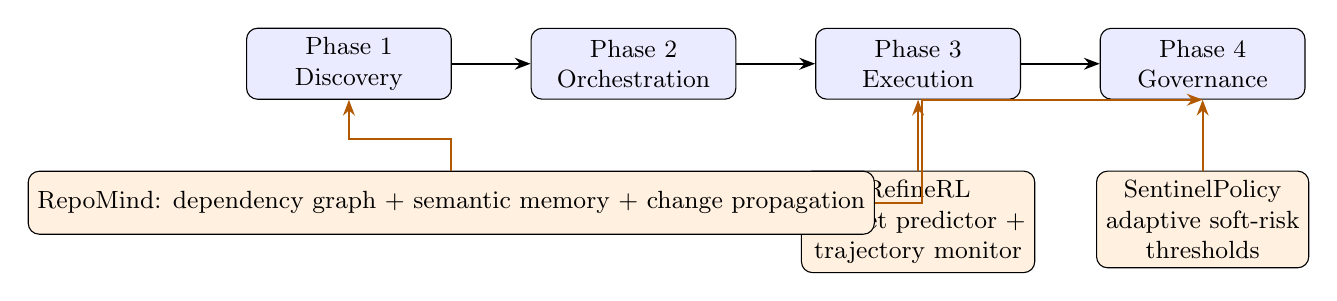
\begin{tikzpicture}[
  phase/.style={draw, rounded corners, minimum height=0.9cm, minimum width=2.6cm, align=center, font=\small, fill=blue!8},
  ext/.style={draw, rounded corners, minimum height=0.8cm, minimum width=2.6cm, align=center, font=\small, fill=orange!12},
  arr/.style={-{Stealth[length=2mm]}, thick}
]
\node[phase] (p1) {Phase 1\\Discovery};
\node[phase, right=1.0cm of p1] (p2) {Phase 2\\Orchestration};
\node[phase, right=1.0cm of p2] (p3) {Phase 3\\Execution};
\node[phase, right=1.0cm of p3] (p4) {Phase 4\\Governance};

\draw[arr] (p1) -- (p2);
\draw[arr] (p2) -- (p3);
\draw[arr] (p3) -- (p4);

\node[ext, below=0.9cm of p3] (rrl) {RefineRL\\budget predictor +\\trajectory monitor};
\node[ext, below=0.9cm of p4] (sp) {SentinelPolicy\\adaptive soft-risk\\thresholds};
\node[ext, below=0.9cm of p1, xshift=1.3cm] (rm) {RepoMind: dependency graph + semantic memory + change propagation};

\draw[arr, orange!70!black] (rrl) -- (p3);
\draw[arr, orange!70!black] (sp) -- (p4);
\draw[arr, orange!70!black] (rm.north) -- ++(0,0.4) -| (p1.south);
\draw[arr, orange!70!black] (rm.east) -- ++(0.6,0) |- (p4.south);
\end{tikzpicture}
\caption{OpsPilot+ extensions layered around the base four-phase pipeline.
Each extension wraps its phase without adding agents or altering the
Coder/Verifier loop's own mechanics; RepoMind spans Phase 1 (graph ingestion)
through Phase 4 (post-verification recording and propagation).}
\label{fig:architecture}
\end{figure*}

Figure \ref{fig:architecture} summarizes how the three extensions attach to
the base pipeline: each wraps a single phase's inputs or outputs rather than
inserting new agents into the phase itself, preserving all four
non-negotiable base-architecture constraints from Section \ref{sec:base}.

\section{Evaluation Methodology}
\label{sec:methodology}

None of the three extensions can be evaluated against a real fleet of human
reviewers, a real multi-week migration, or a real multi-thousand-module
repository within this project's scope, and each extension's own originating
specification anticipates this, prescribing a synthetic-benchmark evaluation
design. We built one benchmark generator per extension.

\textbf{SentinelPolicy} is evaluated with a synthetic-reviewer harness: a
rule-based simulated human reviewer with fixed, category-specific override
probabilities (e.g. frequently overriding rejections on cosmetic
deprecated-API flags, almost never overriding rejections on financial-precision
flags), applied to synthetically generated Java modules with controllable
per-category risk density. Rather than evaluate a single continuous online
run -- which conflates the bandit's own exploration noise with genuine
learning, since a 10-armed decision with a stochastic per-category reward is
dominated by sampling variance at any window short enough to still show a
trend within a few thousand modules -- we use a train/freeze/holdout design:
the bandit learns online over a training stream, exploration is then
disabled (pure exploitation of the learned posterior), and the frozen policy
is scored against a disjoint holdout stream and a matched fresh reviewer
instance, compared to a static uniform-threshold baseline scored on the same
holdout stream.

\textbf{RefineRL} is evaluated on synthetic self-refine trajectories: a
per-module ``true'' convergence iteration is sampled from a distribution
parameterized by the same features the predictor uses (base
$3$--$5$ iterations for typical modules, with additive terms for
embedded-SQL and CICS-handler flags reproducing the source survey's own
reported $3$--$5$ / up to $12$ split), and a corresponding integer-valued
$\delta_t$ trajectory is generated with the initial failure count scaled to
the trajectory's length -- a modeling choice discussed further in Section
\ref{sec:threats}. Three conditions are compared on identical held-out
trajectories: a fixed low budget, a fixed high budget, and RefineRL's
predicted-and-adjusted budget, plus a full fixed-budget sweep to trace the
achievable cost/convergence-rate frontier.

\textbf{RepoMind} is evaluated on a synthetic 80-module repository with 12
shared copybooks (a mix of widely-used ``hub'' copybooks and rarely-used
ones) layered with a directed acyclic call graph, and, critically, per-module
field-level usage tracked separately from the module-level dependency graph
itself. This separation is what makes the evaluation non-tautological: the
graph gives ``who structurally depends on this copybook,'' while ground
truth for a specific injected field-level change is ``who actually
references that field, directly or transitively through a call chain to a
module that does'' -- a strict subset of the structural-dependent set.
Two hundred scenarios inject a breaking change to one randomly chosen field
in one randomly chosen copybook, comparing RepoMind's targeted propagation
against a ``no propagation'' baseline (nothing scheduled) and a ``verify
everything'' baseline (the whole repository scheduled, every time).
Semantic memory recall is evaluated separately, as a standard information-retrieval
task (precision at $k=5$) on a synthetic 150-entry decision corpus spanning
five topically distinct COBOL-idiom categories, against a random-retrieval
baseline.

\section{Results}
\label{sec:results}

\subsection{SentinelPolicy}

Table \ref{tab:sentinel} reports the frozen-policy holdout comparison (5{,}000
training modules, 1{,}200 disjoint holdout modules, static baseline threshold
$0.25$).

\begin{table}[t]
\centering
\caption{SentinelPolicy: static threshold vs. adaptive policy (holdout, frozen)}
\label{tab:sentinel}
\begin{tabular}{@{}lrr@{}}
\toprule
Metric & Static ($t{=}0.25$) & SentinelPolicy \\
\midrule
Flag rate & 47.6\% & 12.8\% \\
Wasted-escalation rate & 10.5\% & \textbf{0.5\%} \\
Override rate given flagged & 22.1\% & 3.9\% \\
Miss rate given approved & 5.9\% & 5.2\% \\
Hard-constraint catch rate & 100\% & 100\% \\
\bottomrule
\end{tabular}
\end{table}

Wasted-escalation rate -- flagged decisions the simulated human ultimately
overrode, the direct operationalization of ``guardrail stagnation'' --
fell 95.3\% relative to the static baseline, while the hard-constraint layer
caught 100\% of injected violations under both conditions, confirming the
adaptive layer never weakens the non-negotiable backstop. This held across a
sweep of static-baseline thresholds from $0.15$ to $0.35$ (relative reduction
range: 86.4\%--97.1\%) and across independent training/holdout seed pairs
(92.1\%--97.7\%), indicating the result is not an artifact of a favorably
chosen baseline or a lucky seed. Figure \ref{fig:sentinel} shows the online
training curve and the frozen-policy holdout comparison.

\begin{figure}[t]
\centering
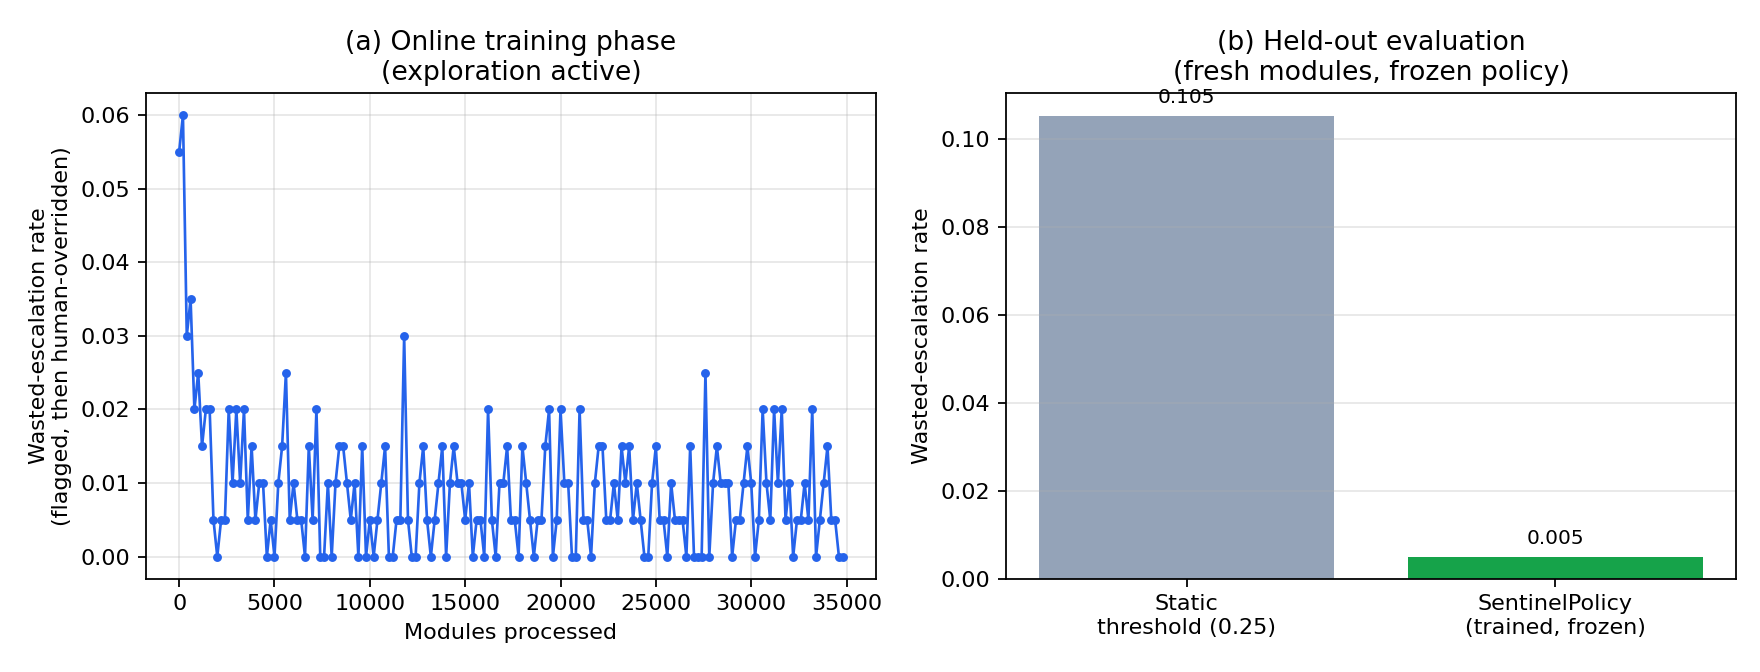
\includegraphics[width=\linewidth]{figures/wasted_escalation_rate.png}
\caption{SentinelPolicy. (a) Online training-phase wasted-escalation rate,
windowed, with active exploration -- noisy by construction, trending down.
(b) Frozen-policy holdout comparison against the static baseline on a
disjoint stream.}
\label{fig:sentinel}
\end{figure}

\subsection{RefineRL}

Table \ref{tab:refinerl} compares fixed-low, fixed-high, and RefineRL on 600
held-out synthetic trajectories (predictor trained on 1{,}500 disjoint
trajectories).

\begin{table}[t]
\centering
\caption{RefineRL vs.\ fixed iteration budgets (600 held-out modules)}
\label{tab:refinerl}
\begin{tabular}{@{}lrrr@{}}
\toprule
Condition & Avg.\ iter./mod. & Converg.\ rate & Premature esc.\ \\
\midrule
Fixed low ($B{=}4$) & 3.91 & 26.5\% & 73.5\% \\
Fixed high ($B{=}12$) & 6.53 & 96.9\% & 3.1\% \\
RefineRL (adaptive) & 6.31 & 88.1\% & 11.9\% \\
\bottomrule
\end{tabular}
\end{table}

RefineRL lands between the two fixed extremes on cost and closer to
fixed-high on convergence rate, and on genuinely unconvergeable modules
specifically -- the case a plateau detector should help most -- it stops
after an average of 8.4 iterations versus fixed-high's 12. But the more
informative comparison is against the achievable frontier traced by sweeping
the fixed budget itself (Figure \ref{fig:refinerl}): at matched cost
($\approx 6.3$ average iterations), a well-chosen single fixed budget
($B{=}9$--$10$) is competitive with, and in this specific synthetic
population's aggregate numbers modestly ahead of, RefineRL's convergence
rate. We report this without reframing it: on this benchmark, RefineRL does
not establish outright Pareto dominance over every fixed choice. What it
does establish is a policy that does not require already knowing which fixed
value is close to optimal for a given (and potentially shifting) module
population, and materially better worst-case behavior at both extremes --
far fewer premature escalations than a conservatively low fixed budget, and
far less wasted iteration spend on modules that were never going to converge
than a conservatively high one.

\begin{figure}[t]
\centering
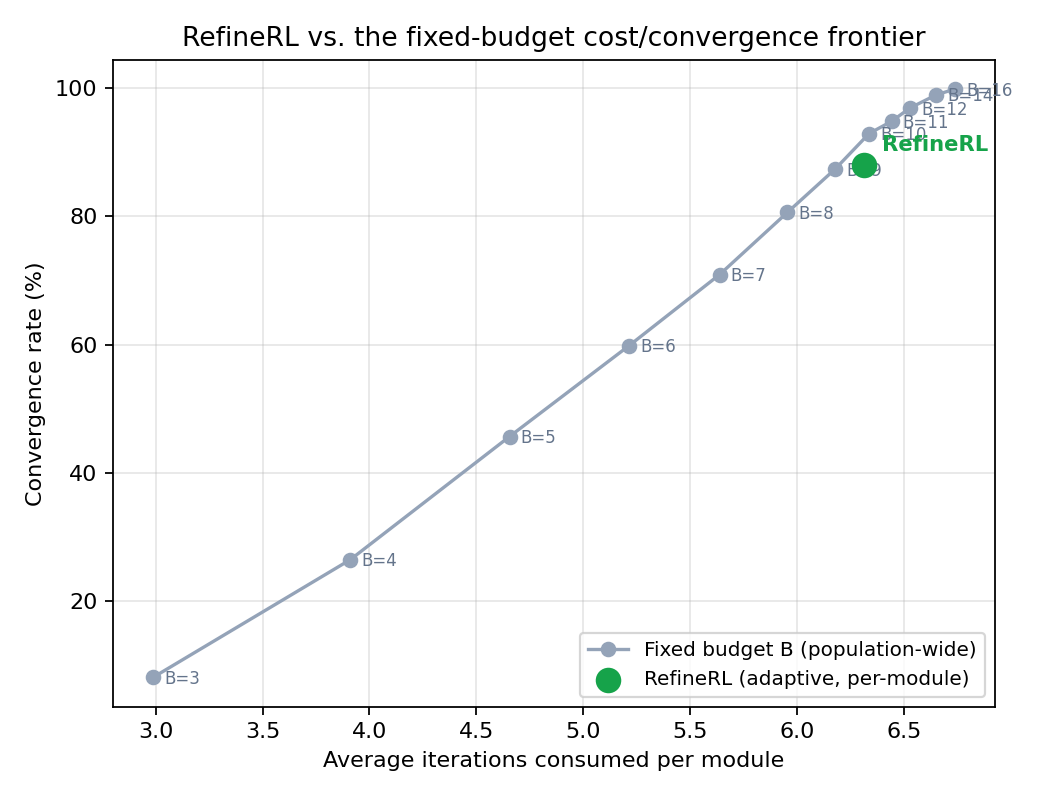
\includegraphics[width=\linewidth]{figures/frontier.png}
\caption{RefineRL (adaptive, per-module) plotted against the cost/convergence
frontier traced by fixed population-wide budgets $B \in \{3,\ldots,16\}$ on
the same held-out modules.}
\label{fig:refinerl}
\end{figure}

\subsection{RepoMind}

Table \ref{tab:repomind} reports propagation results across 200 injected
field-level breaking-change scenarios on the synthetic 80-module repository.

\begin{table}[t]
\centering
\caption{RepoMind change propagation (80-module synthetic repo, 200 scenarios)}
\label{tab:repomind}
\begin{tabular}{@{}lrr@{}}
\toprule
Condition & Recall & Avg.\ modules flagged \\
\midrule
No propagation (manual) & 0\% & 0.0 \\
Verify everything & 100\% & 80.0 \\
RepoMind (targeted) & \textbf{100\%} & \textbf{26.3} \\
\bottomrule
\end{tabular}
\end{table}

RepoMind achieves 100\% recall of truly-impacted modules -- guaranteed by
construction, since the graph traversal is a conservative superset of the
field-level ground truth -- while checking 67.1\% fewer modules than
re-verifying the entire repository (Figure \ref{fig:repomind}). Precision on
non-trivial scenarios (44.8\%) meaningfully exceeds the brute-force
baseline's (17.5\%), the expected profile for a safety-conservative
propagation policy: never miss a truly-affected module, narrow the search
space substantially rather than perfectly. Separately, semantic memory
recall achieved precision@5 of $1.00$ against a random-retrieval baseline of
$0.21$ (topic base rate $0.20$) on the synthetic decision corpus -- a result
we caveat rather than present unqualified, since the synthetic corpus's
topically distinct vocabulary makes this an easier retrieval task than a
production system with noisier, more overlapping rationale text would face.

\begin{figure}[t]
\centering
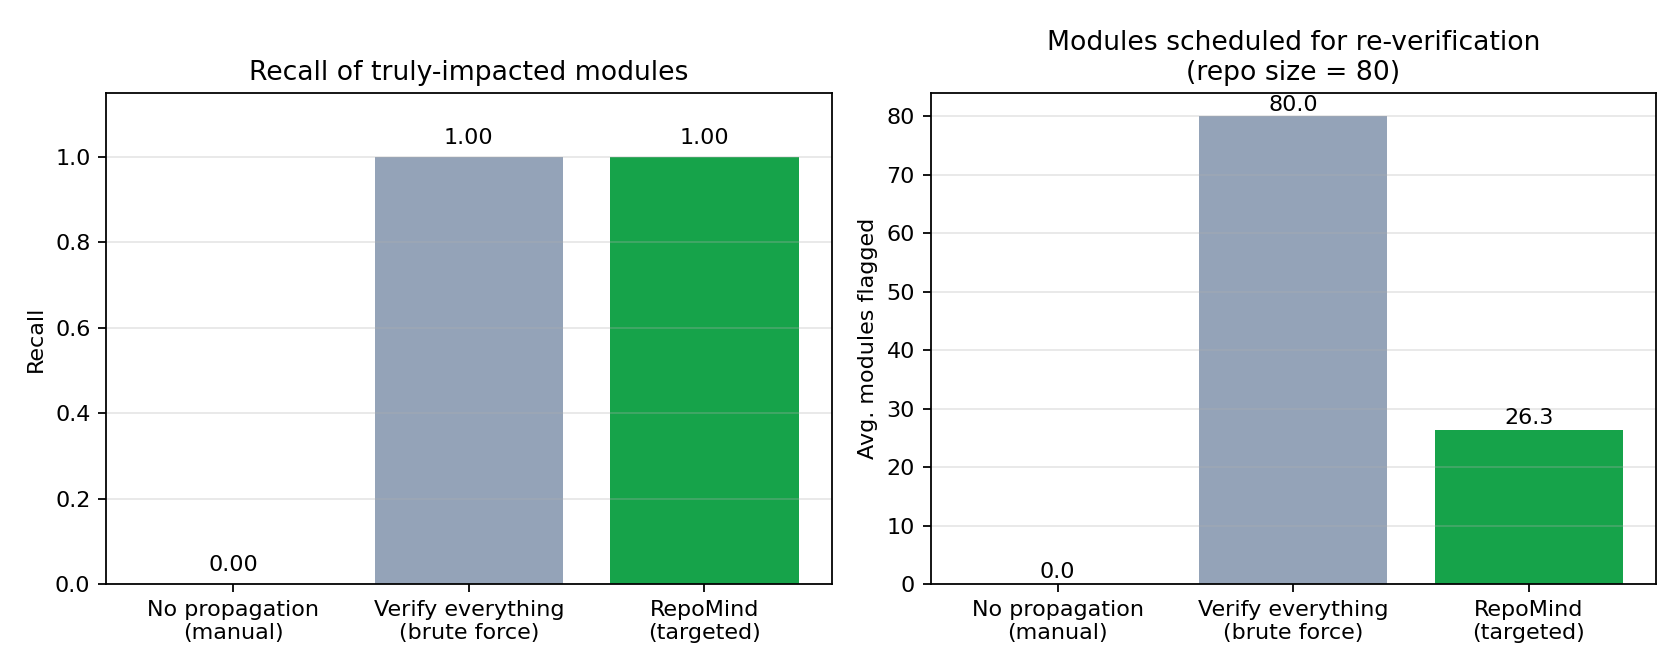
\includegraphics[width=\linewidth]{figures/propagation_comparison.png}
\caption{RepoMind vs.\ no-propagation and verify-everything baselines: recall
of truly-impacted modules (left) and average modules scheduled for
re-verification out of an 80-module repository (right).}
\label{fig:repomind}
\end{figure}

\section{Threats to Validity}
\label{sec:threats}

\textbf{All evaluation is synthetic.} No real human reviewers, no real
multi-week migration, no real multi-thousand-module legacy repository. Every
result in Section \ref{sec:results} is a mechanism test -- does the algorithm
behave correctly and usefully under a plausible, code-generated proxy for
the real distribution -- not a field result. Each extension's originating
specification anticipates and prescribes exactly this kind of synthetic
evaluation given the same constraint, but the gap between synthetic and
field validity remains real and unclosed by this work.

\textbf{The underlying Coder/Verifier loop is a deterministic offline
stand-in, not a live LLM.} This environment has no LLM API access. All three
extensions operate on the loop's inputs, outputs, and control flow (features,
verifier failure counts, generated code text, dependency edges) rather than
on model internals, so the mechanisms themselves are agnostic to whether a
real LLM or the deterministic stand-in produced those outputs -- but no
result here demonstrates behavior under real model variance or real model
failure modes.

\textbf{Three implementation bugs, found and fixed during development, are
reported here rather than silently corrected}, because each is the kind of
mistake that produces a misleadingly clean-looking wrong result rather than
an obviously broken one, and each is now covered by a regression test.
First, an early version of SentinelPolicy's threshold ladder had its lowest
candidate threshold numerically equal to the escalation margin, meaning
code with a risk score of exactly zero -- entirely clean code -- could never
register as APPROVE at that threshold; fixed by keeping the lowest candidate
comfortably above the margin. Second, and more consequential: an early
version aggregated a module's per-category human dispositions into a single
AND'd boolean before recording bandit reward, which let one flagged,
unrelated category suppress the reward signal for every other, well-calibrated
category in the same decision -- this was the direct cause of an early result
that showed the adaptive policy performing \emph{worse} than the static
baseline, which on inspection was a labeling bug, not a genuine negative
result. Third, RefineRL's synthetic trajectory generator could, before a
fix, let injected Gaussian noise round an intermediate failure count down to
zero before the trajectory's own declared true convergence iteration,
making the observable data inconsistent with its own ground truth label.
We report these not to claim the current implementation is bug-free -- it
is not verifiably so -- but because a paper claiming empirical rigor should
show its evaluation code was actually scrutinized, not merely run once.

\textbf{RepoMind's precision/recall result for propagation is true by
construction}, not an empirical finding subject to being wrong: a
conservative graph traversal that walks the same edges the ground truth is
defined from cannot fail to achieve full recall. The empirically meaningful
number is the scope-reduction percentage, not the recall figure, and we
present it that way in Table \ref{tab:repomind} and Section
\ref{sec:results} rather than foreground recall as if it were surprising.

\textbf{RefineRL's near-frontier result depends on synthetic reward-model
assumptions} -- specifically, that a trajectory's initial failure count
scales with its ultimate convergence length. We chose this scaling
deliberately, because without it a plateau detector operating on a
low-cardinality integer signal cannot distinguish a genuinely stalled module
from a slowly-but-genuinely-converging one within any practically short
detection window, and we verified this failure mode directly during
development before adopting the fix (Section \ref{sec:threats}, third bug).
But the scaling choice is a modeling assumption, not a measured property of
real Verifier failure counts, and a different assumption could plausibly
shift where RefineRL sits relative to the fixed-budget frontier.

\section{Future Work}
\label{sec:future}

Beyond the near-term extensions in Section \ref{sec:scope} (asymmetric,
sign-off-gated threshold loosening for SentinelPolicy; a model-tier routing
extension evaluable with the same offline-simulation methodology used for
RefineRL; a real embedding backend for RepoMind's semantic memory once
network access to one is available), the more consequential open question is
closing the synthetic-to-real gap directly identified in Section
\ref{sec:threats}: a small-scale pilot with actual human reviewers providing
real override decisions for SentinelPolicy, actual logged self-refine
trajectories from a real LLM Coder/Verifier pair for RefineRL, and a real,
smaller-scale legacy repository with hand-labeled ground-truth dependencies
for RepoMind, would let each extension's synthetic-benchmark result be
checked against, rather than merely modeled after, the phenomenon it targets.

\section{Conclusion}
\label{sec:conclusion}

We implemented OpsPilot as working code and extended it with three additive
subsystems -- SentinelPolicy, RefineRL, RepoMind -- each closing a gap the
source survey names as open and unbuilt, each evaluated with reproducible
experiments against principled baselines. Two of the three produce clean,
substantial improvements on their synthetic benchmarks: a 95.3\% relative
reduction in wasted guardrail escalations with the hard-constraint backstop
fully intact, and 100\% recall of truly-impacted modules at a 67\% reduction
in re-verification scope. The third, RefineRL, produces a genuinely more
qualified result -- competitive with, rather than dominant over, a
well-tuned fixed budget on this benchmark's aggregate numbers -- which we
report as such rather than reframe, in the same evidentiary spirit the
source survey applies to its own headline figures. Taken together with an
explicit account of which further directions were considered and why they
were not pursued here, we hope this implementation gives the source survey's
named gaps their first concrete, testable answers, imperfect and synthetic
as those answers currently are.

\section*{Availability}
Source code, unit tests, evaluation harnesses, and the exact configuration
used to produce every number and figure in this paper are included in the
accompanying project repository, along with an implementation-notes document
recording the scope decisions summarized in Section \ref{sec:scope} and the
bugs discussed in Section \ref{sec:threats} in full detail.

\begin{thebibliography}{00}

\bibitem{survey} S. V. Togarshi, S. S. Naik, S. I. M., S. Arya, and T.
Naquash, ``Multi-Agent Orchestration for Legacy Toolchain Modernization: A
Comprehensive Survey,'' HKBK Institute of Technology, 2026.

\bibitem{autogen} Q. Wu \emph{et al.}, ``AutoGen: Enabling Next-Gen LLM
Applications via Multi-Agent Conversations,'' in \emph{Proc. Conf. Lang.
Model. (COLM)}, 2024.

\bibitem{guardrails} A. Mishra, ``Understanding AI Guardrails: Concepts,
Models, and Methods,'' \emph{IJIRMPS}, vol. 13, no. 1, Jan.--Feb. 2025.

\bibitem{selfrefine} A. Madaan \emph{et al.}, ``Self-Refine: Iterative
Refinement with Self-Feedback,'' in \emph{Advances in Neural Information
Processing Systems (NeurIPS)}, vol. 36, 2023.

\bibitem{reflexion} N. Shinn, F. Cassano, A. Gopinath, K. Narasimhan, and S.
Yao, ``Reflexion: Language Agents with Verbal Reinforcement Learning,'' in
\emph{Advances in Neural Information Processing Systems (NeurIPS)}, vol. 36,
2023.

\bibitem{react} S. Yao \emph{et al.}, ``ReAct: Synergizing Reasoning and
Acting in Language Models,'' in \emph{Proc. Int. Conf. Learn. Repr. (ICLR)},
2023.

\bibitem{ucb} P. Auer, ``Using Confidence Bounds for Exploitation-Exploration
Trade-offs,'' \emph{Journal of Machine Learning Research}, vol. 3, pp.
397--422, 2002.

\bibitem{thompson1933} W. R. Thompson, ``On the Likelihood that One Unknown
Probability Exceeds Another in View of the Evidence of Two Samples,''
\emph{Biometrika}, vol. 25, no. 3/4, pp. 285--294, 1933.

\bibitem{thompsontutorial} D. J. Russo, B. Van Roy, A. Kazerouni, I. Osband,
and Z. Wen, ``A Tutorial on Thompson Sampling,'' \emph{Foundations and
Trends in Machine Learning}, vol. 11, no. 1, pp. 1--96, 2018.

\bibitem{linucb} L. Li, W. Chu, J. Langford, and R. E. Schapire, ``A
Contextual-Bandit Approach to Personalized News Article Recommendation,'' in
\emph{Proc. 19th Int. Conf. World Wide Web (WWW)}, 2010, pp. 661--670.

\end{thebibliography}

\end{document}
